\documentclass[aspectratio=169,11pt]{beamer}

\usepackage{graphicx}
\usepackage{newtxtext,newtxmath} % Times New Roman-like font, Overleaf-safe
\usepackage{tikz}
\usetikzlibrary{positioning,arrows.meta}
\usepackage{xcolor}
\usepackage{booktabs}
\usepackage{tabularx}
\usepackage{array}
\usepackage{ragged2e}

\definecolor{GEUBlue}{RGB}{20,55,105}
\definecolor{GEULightBlue}{RGB}{238,244,251}
\definecolor{GEUGrey}{RGB}{90,90,90}
\definecolor{GEULightGrey}{RGB}{245,246,248}

\usetheme{default}
\setbeamertemplate{navigation symbols}{}
\setbeamertemplate{blocks}[rounded][shadow=false]
\setbeamercolor{normal text}{fg=black,bg=white}
\setbeamercolor{frametitle}{fg=GEUBlue}
\setbeamercolor{structure}{fg=GEUBlue}
\setbeamercolor{block title}{fg=GEUBlue,bg=GEULightBlue}
\setbeamercolor{block body}{fg=black,bg=GEULightBlue}
\setbeamerfont{frametitle}{size=\Large,series=\bfseries}

% Put the logo file in the same Overleaf project folder.
% Change only this filename if your uploaded logo has a different name.
\newcommand{\GEULogo}{graphic.jpeg}
\graphicspath{{./}}

% Keep all slide content above the footer.
\setlength{\footskip}{0.18cm}

\setbeamertemplate{headline}{%
  \begin{tikzpicture}[remember picture,overlay]
    \node[anchor=north east,xshift=-0.30cm,yshift=-0.12cm]
      at (current page.north east)
      {\includegraphics[height=0.62cm]{\GEULogo}};
  \end{tikzpicture}
  \vspace{0.72cm}
}

\setbeamertemplate{frametitle}{%
  \vspace{0.03cm}
  \insertframetitle\par
  \vspace{0.04cm}
  \textcolor{GEUBlue}{\rule{\textwidth}{0.9pt}}
  \vspace{0.03cm}
}

\setbeamertemplate{footline}{%
  \leavevmode
  \hbox{%
  \begin{beamercolorbox}[wd=.82\paperwidth,ht=0.32cm,dp=0.10cm,leftskip=.3cm]{author in head/foot}
    \tiny Department of Computer Science \& Engineering | Graphic Era (Deemed to be University)
  \end{beamercolorbox}%
  \begin{beamercolorbox}[wd=.18\paperwidth,ht=0.32cm,dp=0.10cm,rightskip=.3cm]{date in head/foot}
    \hfill\tiny\insertframenumber/\inserttotalframenumber
  \end{beamercolorbox}}
}

\begin{document}

% =========================================================
% SLIDE 1
% =========================================================
\begin{frame}[plain]
\begin{tikzpicture}[remember picture,overlay]
\draw[GEUBlue,line width=3pt]
  (current page.north west) -- (current page.north east);

\node[anchor=north east,xshift=-0.45cm,yshift=-0.35cm]
  at (current page.north east)
  {\includegraphics[height=1.0cm]{\GEULogo}};

\node[align=center,text width=.84\paperwidth]
  at ([yshift=.25cm]current page.center)
{
{\color{GEUBlue}\fontsize{26}{30}\selectfont\bfseries PROJECT-BASED LEARNING}\\[3mm]
{\fontsize{18}{22}\selectfont PHASE-I EVALUATION}\\[7mm]
{\color{GEUGrey}\Large\bfseries SOUNDSYNC : Smart Music Player}\\[3mm]
{\color{GEUBlue}\normalsize Team ID: DSCPP-III-2026-T201}
};

\node[align=center,anchor=south,yshift=.42cm]
  at (current page.south)
{
\bfseries Department of Computer Science \& Engineering\\
Graphic Era (Deemed to be University), Dehradun\\[-1mm]
\scriptsize Academic Session 2026--27
};
\end{tikzpicture}
\end{frame}

% =========================================================
% SLIDE 2
% =========================================================
\begin{frame}{Team \& Mentor Details}
\begin{columns}[T,totalwidth=\textwidth]\small

\column{.47\textwidth}
\begin{block}{Team Information}
\begin{tabular}{@{}ll@{}}
\textbf{Team ID:} & DSCPP-III-2026-T201\\
\textbf{Semester:} & 3rd\\
\textbf{Section:} & K, E, ML-1\\
\textbf{Domain:} & DSA \& OOPs with C++
\end{tabular}
\end{block}

\column{.47\textwidth}
\begin{block}{Team Members}
1. Sanya Goel -- 2510010795\\[1mm]
2. Manvi Arora -- 2510010232\\[1mm]
3. Eshu Ram -- 2510011472
\end{block}

\end{columns}

\vspace{2mm}
\begin{columns}[T,totalwidth=\textwidth]
\column{.47\textwidth}
\begin{block}{Mentor}
\textbf{Mr. Abhinav Kotnala}
\end{block}
\column{.47\textwidth}
\begin{block}{Interactions}
\textbf{Interactions completed:} 3
\end{block}
\end{columns}
\end{frame}

% =========================================================
% SLIDE 3
% =========================================================
\begin{frame}{Problem Statement \& Motivation}

\begin{block}{Problem Statement}
Our project solves the real-world problem of managing growing personal
music libraries by providing an organized system for fast song access,
personalized playlist management, and efficient music playback.
\end{block}

\vspace{2mm}

\begin{columns}[T,totalwidth=\textwidth]

\column{.48\textwidth}
\textbf{\color{GEUBlue}Motivation}
\begin{itemize}\itemsep4pt
\item Limited playlist management
\item Saves time and improves accessibility
\item Scattered songs make searching difficult
\end{itemize}

\column{.48\textwidth}
\textbf{\color{GEUBlue}Target Users / Stakeholders}
\begin{itemize}\itemsep4pt
\item Music listeners
\item Students
\item Developers and mentors
\item Easy access and efficient playback
\end{itemize}

\end{columns}
\end{frame}

% =========================================================
% SLIDE 4
% =========================================================
\begin{frame}{Objectives}

\textbf{\color{GEUBlue}Project Objectives}
\vspace{2mm}

\begin{enumerate}\itemsep5pt
\item Develop a simple smart music management system.
\item Implement song search, playback, and playlist management.
\item Integrate C++ concepts, OOPs, and data structures.
\item Evaluate the system using functional test cases.
\item Demonstrate practical use and future scalability.
\end{enumerate}

\vfill

\begin{center}
\colorbox{GEULightBlue}{%
\parbox{.80\textwidth}{\centering
\textbf{Key Objective:}
To provide fast song access and efficient playlist management
for a personal music playlist.}}
\end{center}

\end{frame}

% =========================================================
% SLIDE 5
% =========================================================
\begin{frame}{Proposed Solution}

\begin{columns}[T,totalwidth=\textwidth]

\column{.48\textwidth}
\textbf{\color{GEUBlue}Proposed Approach}
\begin{enumerate}\itemsep3pt
\item User selects songs and enters playlist details.
\item Search, sort, add, delete, and play songs using data structures.
\item Manage songs, playlists, and playback based on user choices.
\item Store song details and playlists using files/local storage.
\item Display songs, playlists, and playback status through a simple UI.
\end{enumerate}

\column{.48\textwidth}
\textbf{\color{GEUBlue}Key Features}
\begin{itemize}\itemsep4pt
\item Song Search \& Selection
\item Music Playback
\item Playlist Creation \& Management
\item Add / Delete Songs
\item Song Sorting \& Organization
\end{itemize}

\end{columns}
\end{frame}

% =========================================================
% SLIDE 6
% =========================================================
\begin{frame}{Integration of PBL Course Concepts}

\scriptsize
\begin{center}
\renewcommand{\arraystretch}{1.35}

\begin{tabularx}{.96\textwidth}
{@{}>{\bfseries}p{3.2cm}X p{3.0cm}@{}}
\toprule
Course & Concepts Applied & Project Module\\
\midrule
Data Structures in C &
Arrays, Linked Lists, Trees, Graphs, Hashing, Stacks, Queues &
Songs \& Playlist Management\\

OOPs with C++ &
Classes, Objects, Inheritance, Polymorphism, STL &
Music Player \& User Management\\
\bottomrule
\end{tabularx}
\end{center}

\vfill

\begin{center}
\colorbox{GEULightBlue}{%
\parbox{.86\textwidth}{\centering
\textbf{Requirement:}
Data Structures efficiently manage music data, while OOPs provides
a modular and reusable structure for the music player system.}}
\end{center}

\end{frame}

% =========================================================
% SLIDE 7
% =========================================================
\begin{frame}{System Architecture / Workflow}

\begin{center}
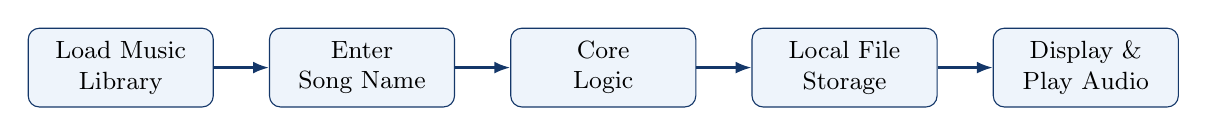
\begin{tikzpicture}[
node distance=7mm,
box/.style={
rectangle,rounded corners,draw=GEUBlue,fill=GEULightBlue,
minimum width=2.35cm,minimum height=10mm,align=center,font=\small
},
arrow/.style={-{Latex[length=2mm]},thick,draw=GEUBlue}
]

\node[box] (a) {Load Music\\Library};
\node[box,right=of a] (b) {Enter\\Song Name};
\node[box,right=of b] (c) {Core\\Logic};
\node[box,right=of c] (d) {Local File\\Storage};
\node[box,right=of d] (e) {Display \&\\Play Audio};

\draw[arrow] (a)--(b);
\draw[arrow] (b)--(c);
\draw[arrow] (c)--(d);
\draw[arrow] (d)--(e);

\end{tikzpicture}
\end{center}

\vspace{1.0mm}

{\footnotesize
\begin{columns}[T,totalwidth=\textwidth]

\column{.48\textwidth}
\textbf{\color{GEUBlue}Major Components}
\begin{itemize}\itemsep1.5pt\parskip0pt
\item Music Library Module -- Stores and manages songs using arrays/vectors.
\item Playlist Module -- Creates and manages playlists using linked lists.
\item Music Player Module -- Handles play, next, previous and song queue using stack and queue.
\end{itemize}

\column{.48\textwidth}
\textbf{\color{GEUBlue}Data / Control Flow}
\begin{itemize}\itemsep1.5pt\parskip0pt
\item User selects/searches a song -- system processes the request.
\item Song data is retrieved from the music library and playlist.
\item Player controls the selected song and manages the queue.
\item Output -- song information, playlist and currently playing songs.
\end{itemize}

\end{columns}}
\end{frame}

% =========================================================
% SLIDE 8
% =========================================================
\begin{frame}{Technology Stack \& Methodology}

\begin{columns}[T,totalwidth=\textwidth]

\column{.48\textwidth}
\begin{block}{Technology Stack}
\begin{itemize}\itemsep1pt\parskip0pt
\item Programming: C / C++ / Python
\item Database: MySQL / File Storage
\item Tools / Framework: SFML (Audio)
\item IDE: Visual Studio Code
\item Version Control: Git / GitHub
\end{itemize}
\end{block}

\column{.48\textwidth}
\begin{block}{Development Methodology}
\begin{enumerate}\itemsep1pt\parskip0pt
\item Identify user needs and project requirements.
\item Design modules, data structures, and workflow.
\item Develop the music player using C/C++ and SFML.
\item Test playback, searching, playlists, and other functions.
\item Check performance, usability, and overall functionality.
\end{enumerate}
\end{block}

\end{columns}
\end{frame}

% =========================================================
% SLIDE 9
% =========================================================
\begin{frame}{Initial Progress \& Team Contribution}

\begin{columns}[T,totalwidth=\textwidth]

\column{.43\textwidth}
\textbf{\color{GEUBlue}Progress Achieved}
\begin{itemize}\itemsep4pt
\item Scope defined and predefined collection of songs identified.
\item Data structures selected for library, playlists, history, queue and search.
\item C++ class/module structure planned.
\item High-level system architecture and workflow prepared.
\end{itemize}

\column{.54\textwidth}
\textbf{\color{GEUBlue}Individual Contribution}
\vspace{2mm}

\scriptsize
\begin{tabularx}{\textwidth}{@{}p{1.65cm}p{2.15cm}X@{}}
\toprule
Member & Role & Contribution\\
\midrule
Sanya & Team Lead &
Task coordination, overall system development\\
Manvi & Developer &
Project report documentation and formatting\\
Eshu & Developer/Docs &
Testing and debugging\\
\bottomrule
\end{tabularx}

\end{columns}
\end{frame}

% =========================================================
% SLIDE 10
% =========================================================
\begin{frame}{Roadmap, Expected Outcomes \& References}

% Use compact spacing only on this slide so that nothing reaches the footer.
\setlength{\parskip}{0pt}
\setlength{\itemsep}{0pt}

\begin{columns}[T,totalwidth=\textwidth]

% ---------------------------------------------------------
% LEFT COLUMN
% ---------------------------------------------------------
\column{.47\textwidth}

{\small
\textbf{\color{GEUBlue}Roadmap}

\vspace{1mm}
\begin{enumerate}
    \setlength{\itemsep}{2pt}
    \setlength{\parskip}{0pt}
    \item Phase-I: Proposal \& System Design
    \item Phase-II: C/C++ Development
    \item Phase-III: Final Implementation, Testing,
          UI/Audio Integration
\end{enumerate}

\vspace{2mm}
\textbf{\color{GEUBlue}Expected Outcomes}

\vspace{1mm}
\begin{itemize}
    \setlength{\itemsep}{2pt}
    \setlength{\parskip}{0pt}
    \item Working music player prototype
    \item Song and playlist management
    \item Fast song search
    \item Practical use of DSA and OOPs
    \item Scope for future scalability
\end{itemize}
}

% ---------------------------------------------------------
% RIGHT COLUMN
% ---------------------------------------------------------
\column{.47\textwidth}

{\small
\textbf{\color{GEUBlue}References}

\vspace{1mm}
\begin{enumerate}
    \setlength{\itemsep}{3pt}
    \setlength{\parskip}{0pt}
    \item Spotify official documentation
    \item C++ documentation
    \item DSA/OOP textbook
    \item GitHub repositories
    \item AI Assistance -- ChatGPT, Claude
    \item LaTeX documentation
\end{enumerate}
}

\vfill

\begin{center}
\colorbox{GEUBlue}{%
\parbox{.82\linewidth}{%
\centering
\color{white}
\textbf{\large Thank You}\\[1mm]
\normalsize Questions \& Suggestions}}
\end{center}

\end{columns}
\end{frame}

\end{document}